\section{System Design}
\label{sec:system_design}
The system design is a hardware/software co-design framework for low-power AI deployment. This architecture allows design exploration of dedicated hardware for TensorFlow Lite on low-cost embedded FPGAs.

\subsection{Base embedded system architecture}
The base embedded system architecture implements a cooperative hardware-software platform. \Fig{fig:system_architecture} illustrates the top-level hardware architecture. The TPs execute low-level tensor operations delegated from the embedded CPU. The TPs employ AXI-Lite interface for configuration and AXI-Stream interfaces via Direct Memory Access (DMA) for data movement from DDR memory. Each TP asserts an interrupt flag once the job/transaction is complete. Interrupt events are handled by the embedded CPU to collect results and start a new transaction. The hardware architecture can resize its resource utilization and energy consumption by customizing the TPs prior to the hardware synthesis.
\begin{figure}[t!]
	\centering
	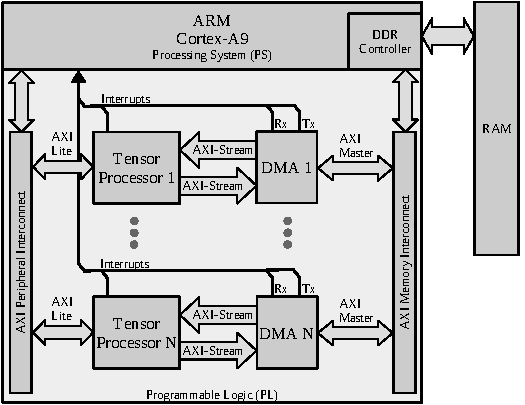
\includegraphics[width=0.5\textwidth]{../figures/system_design.pdf}
	\caption{Base embedded system architecture.}
	\label{fig:system_architecture}
\end{figure}
\subsection{Tensor processor}
The TP is a dedicated hardware module to compute tensor operations. The hardware architecture is described in \fig{fig:accelerator}. This architecture implements high performance communication with AXI-Stream, direct CPU communication with AXI-Lite, and on-chip storage utilizing BRAM. This hardware architecture is implemented with high-level synthesis (HLS). The tensor operations are implemented based on the C++ TensorFlow Lite micro kernels.

The TP is an extensible hardware module that executes low-level tensor operations. In this paper, we focus on the \emph{Conv2D} tensor operator that executes inference of convolution layers.

\begin{figure}[t!]
	\centering
	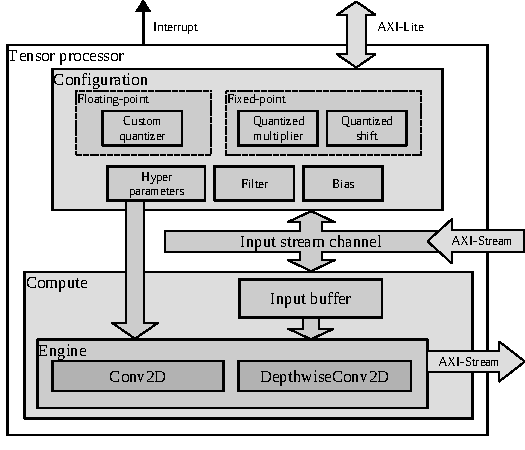
\includegraphics[width=0.5\textwidth]{../figures/accelerator.pdf}
	\caption{Hardware architecture of the proposed tensor processor.}
	\label{fig:accelerator}
\end{figure}
\subsubsection{\textbf{Modes of operation}}
The TP has two modes of operation: \emph{configuration} and \emph{execution}.
\begin{itemize}
	\item In \emph{configuration} mode, the TP receives the tensor operation ID for \emph{Conv2D} and hyperparameters: stride, dilation, padding, offset, activation, depth-multiplier, input shape, filter shape, bias shape, and output shape. Afterwards, the TP receives filter and bias tensors, which are locally stored in BRAM.
	
	\item In \emph{execution} mode, the TP executes the tensor operation according to the hyperparameters given in the configuration mode. During execution, the input and output tensors are moved from/to the DDR memory via DMA.
\end{itemize}
\subsubsection{\textbf{Dot-product with hybrid floating-point}}
\label{sec:dot_product}
We implement the floating-point computation adopting the dot-product with hybrid custom floating-point\cite{nevarez2021accelerating}. The hardware dot-product is illustrated in \Fig{fig:dot_product}. This approach: (1) denormalizes input values, (2) executes computation with integer format for exponent and mantissa, and finally, (3) it normalizes the result into IEEE 754 format, see \Fig{fig:dot_product_hybrid}. 

Rather than a parallelized structure, this is a pipelined hardware design suitable for resource-limited devices. The latency in clock cycles of this hardware module is defined by \equ{eq:dot_custom_float_latency}, where $N$ is the vector length. The latency equations are obtained from the general pipelined hardware latency formula: $L=\left(N-1\right)II+IL$, where $II$ is the initiation interval (\fig{fig:dot_product_hybrid}(a)), and $IL$ is the iteration latency (\fig{fig:dot_product_hybrid}(b)). Both $II$ and $IL$ are obtained from the high-level synthesis results. Both the exponent and mantissa bit widths of the filter and bias buffers are set to a 4-bit exponent and a 1-bit mantissa (E4M1), which corresponds to float6 quantization.

\begin{eqnarray} \label{eq:dot_custom_float_latency}
L_{hf}=N+7
\end{eqnarray}

\begin{figure}[t!]
	\centering
	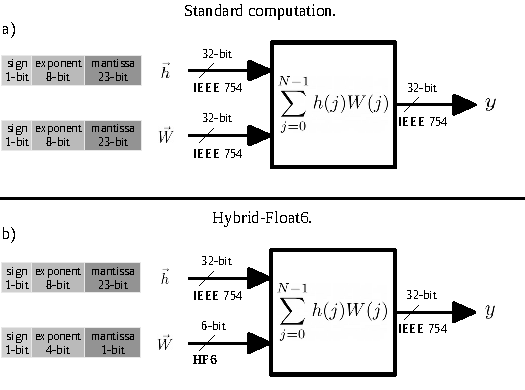
\includegraphics[width=0.5\textwidth]{../figures/dot-product_unit.pdf}
	\caption{Dot-product hardware module with (a) standard floating-point and (b) Hybrid-Float6.}
	\label{fig:dot_product}
\end{figure}

\begin{figure}[t!]
	\centering
	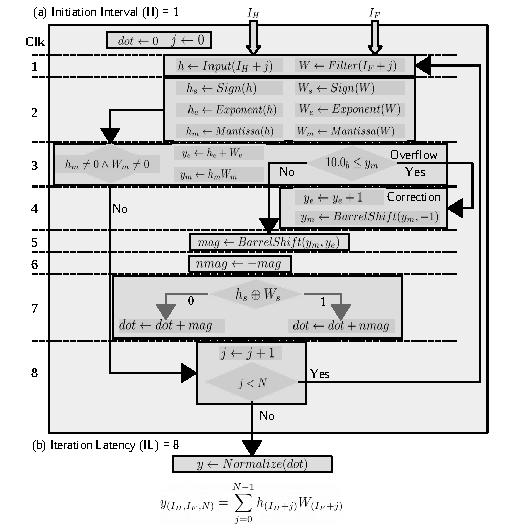
\includegraphics[width=0.5\textwidth]{../figures/dot_product_hybrid.pdf}
	\caption{Pipelined hardware module for vector dot-product with hybrid custom floating-point, (a) exhibits the initiation interval of 1 clock cycle, and (b) presents
		the iteration latency of 8 clock cycles. $I_H$ and $I_F$ represent the input and filter buffer indexes, respectively.}
	\label{fig:dot_product_hybrid}
\end{figure}

\subsubsection{\textbf{On-chip memory utilization}}
The total on-chip memory utilization on the TP is defined by \Equ{eq:tp_memory}, where $Input_{M}$ is the \emph{input buffer}, $Filter_{M}$ is the \emph{filter buffer}, $Bias_{M}$ is the \emph{bias buffer}, and $V_{M}$ represents the local variables required for the design. The on-chip memory buffers are defined in bits. \fig{fig:accelerator_buffers} illustrates the convolution operation utilizing the on-chip memory buffers.

\begin{figure}[t!]
	\centering
	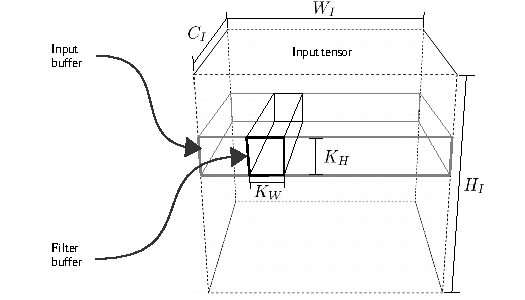
\includegraphics[width=0.5\textwidth]{../figures/accelerator_buffers.pdf}
	\caption{Design parameters for on-chip memory buffers on the TP.}
	\label{fig:accelerator_buffers}
\end{figure}

\begin{eqnarray} \label{eq:tp_memory}
TP_{M}=Input_{M}+Filter_{M}+Bias_{M}+V_{M}
\end{eqnarray}

The memory utilization of \emph{input buffer} is defined by \Equ{eq:input_memory}, where $K_{H}$ is the height of the convolution kernel, $W_{I}$ is the width of the input tensor, $C_{I}$ is the number of input channels, and $BitSize_{I}$ is the bit size of each input tensor element.

\begin{eqnarray} \label{eq:input_memory}
Input_{M}=K_{H}W_{I}C_{I}BitSize_{I}
\end{eqnarray}

The memory utilization of \emph{filter buffer} is defined by \Equ{eq:filter_memory}, where $K_{W}$ and $K_{H}$ are the width and height of the convolution kernel, respectively; $C_{I}$ and $C_{O}$ are the number of input and output channels, respectively; and $BitSize_{F}$ is the bit size of each filter element.

\begin{eqnarray} \label{eq:filter_memory}
Filter_{M}=C_{I}K_{W}K_{H}C_{O}BitSize_{F}
\end{eqnarray}

The memory utilization of \emph{bias buffer} is defined by \Equ{eq:bias_memory}, where $C_{O}$ is the number of output channels, and $BitSize_{B}$ is the bit size of each bias element.

\begin{eqnarray} \label{eq:bias_memory}
Bias_{M}=C_{O}BitSize_{B}
\end{eqnarray}

As a design trade-off, \Equ{eq:channel_in_memory} defines the capacity of output channels based on the given design parameters. The total on-chip memory $TP_{M}$ determines the TP capacity.

\begin{eqnarray} \label{eq:channel_in_memory}
C_{O}=\frac{TP_{M}-V_{M}-K_{H}W_{I}C_{I}BitSize_{I}}{C_{I}K_{W}K_{H}BitSize_{F}+BitSize_{B}}
\end{eqnarray}

The floating-point formats implemented in the TP are defined by $BitSize_F$, $BitSize_B$ and $BitSize_I$. The HF6 defines 6-bits for $BitSize_F$ and $BitSize_B$, and 32-bits for $BitSize_I$. These are design parameters defined before hardware synthesis. This allows fine control of BRAM utilization, which is suitable for resource-limited devices.

\subsection{Quantized aware training}
The quantize-aware training method is an iterative optimization. The custom CNN model is initially trained with early stop monitoring for minimal validation loss, then the CNN model is retrained including the quantization method implemented as a callback function, see \Algo{alg:training}. The quantization method maps the full precision filter and bias values with rounding to the closest representable quantized values, see \Algo{alg:quantize_training}. We have observed that the exponent bit size plays a more predominant influence on the model accuracy than the mantissa bit size. In \cite{lai2017deep}, Lai et al. demonstrated that 4-bit exponent is adequate and consistent across different networks (SqueezeNet, AlexNet, GoogLeNet, VGG-16). In this work, we investigate 4-bit exponent and 1-bit mantissa. This method quantizes the filter and bias tensors of the \emph{Conv2D}. This method is integrated in TensorFlow/Keras framework. On the desktop computer, the resulting quantized parameters are wrapped into the standard floating-point. On the embedded system, the 6-bit floating-point values are extracted and buffered in the on-chip memory of the TP during operation.
\begin{algorithm}[h!]
	\label{alg:training}
	\caption{Training method.}
	\begin{algorithmic}
		\SetAlgoLined
		\renewcommand{\algorithmicrequire}{\textbf{input:}}
		\renewcommand{\algorithmicensure}{\textbf{output:}}
		\REQUIRE $MODEL$ as the CNN.
		\REQUIRE $E_{size}$ as the target exponent bit size.
		\REQUIRE $M_{size}$ as the target mantissa bits size.
		\REQUIRE $D_{train}$ as the training data set.
		\REQUIRE $D_{val}$ as the validation data set.
		\REQUIRE $Acc_d$ as the accuracy degradation threshold.
		\REQUIRE $Loop_{max}$ as the max quantization loop iterations.
		\ENSURE $MODEL$ as the quantized CNN.
		\STATE $Train(MODEL, D_{train}, D_{val})$ // Regular training
		\STATE $acc_i \gets Evaluate(MODEL, D_{val})$ // Benchmark
		\STATE $acc_q \gets 0, loop_c \gets 0$ // Initialize quantize training
		\WHILE {$(acc_q<acc_i - Acc_d) \land (loop_c<Loop_{max})$}
		\STATE // Iterative optimization
		\STATE $callback \gets Quantize(E_{size}, M_{size})$
		\STATE $Train(MODEL, D_{train}, D_{val}, callback)$
		\STATE $acc_q \gets Evaluate(MODEL, D_{val})$
		\STATE $loop_c \gets loop_c + 1$
		\ENDWHILE
	\end{algorithmic}
\end{algorithm}
\begin{algorithm}[h!]
	\label{alg:quantize_training}
	\caption{Custom floating-point quantization method.}
	\begin{algorithmic}
		\SetAlgoLined
		\renewcommand{\algorithmicrequire}{\textbf{input:}}
		\renewcommand{\algorithmicensure}{\textbf{output:}}
		\REQUIRE $MODEL$ as the CNN.
		\REQUIRE $E_{size}$ as the target exponent bit size.
		\REQUIRE $M_{size}$ as the target mantissa bits size.
		\REQUIRE $STDM_{size}$ as the IEEE 754 mantissa bit size.
		\ENSURE $MODEL$ as the quantized CNN.
		\FOR {$layer$ in $MODEL$}
		\IF {$layer$ is $Conv2D$ or $SeparableConv2D$}
		\STATE $filter, bias \gets GetWeights(layer)$
		\FOR {$x$ in $filter$ and $bias$}
			\STATE $sign \gets GetSign(x)$
			\STATE $exp \gets GetExponent(x)$
			\STATE $fullexp \gets 2^{E_{size}-1}-1$ // Get full range value
			\STATE $cman \gets GetCustomMantissa(x, M_{size})$
			\STATE $leftman \gets GetLeftoverMantissa(x, M_{size})$
			\IF {$exp <-fullexp$}
				\STATE$x\gets0$
			\ELSIF{$exp > fullexp$}
				\STATE$x\gets (-1)^{sign}\cdot2^{fullexp}\cdot(1+(1-2^{-M{size}}))$
			\ELSE
				\IF {$2^{STDM_{size}-M_{size}-1}-1<leftman$}
					\STATE $cman \gets cman+1$ // Above halfway
					\IF{$2^{M_{size}}-1<cman$}
					\STATE $cman \gets 0$ // Correct mantissa overflow
					\STATE $exp \gets exp + 1$
					\ENDIF
				\ENDIF
				\STATE // Build custom quantized floating-point value
				\STATE$x\gets (-1)^{sign}\cdot2^{exp}\cdot(1+cman\cdot2^{-M_{size}})$
			\ENDIF
		\ENDFOR
		\STATE $SetWeights(layer, filter, bias)$
		\ENDIF
		\ENDFOR
	\end{algorithmic}
\end{algorithm}
\begin{figure}[t!]
	\centering
	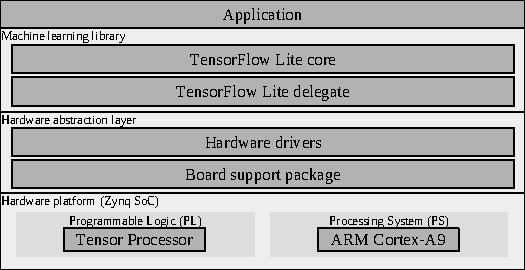
\includegraphics[width=0.5\textwidth]{../figures/sw_stack.pdf}
	\caption{Base embedded software architecture.}
	\label{fig:sw_stack}
\end{figure}
\subsection{Embedded software architecture}
The software architecture is a layered object-oriented application framework written in C++, see \fig{fig:sw_stack}. The main characteristics o the software layers are as follows:
\begin{itemize}
	\item \emph{Application}: As the highest level of abstraction, this layer implements the embedded application logic with the ML library.
	\item \emph{Machine learning library}: This layer consist of TensorFlow Lite micro. This offers a comprehensive high level API that allows ML inference. This provides delegate interfaces for custom hardware accelerators.
	\item \emph{Hardware abstraction layer}: This layer consist of the hardware drivers to handle initialization and runtime operation of the TP and DMA.
\end{itemize}